\documentclass[../thesis.tex]{subfiles}
\begin{document}
\chapter{Organic Light-Emitting Devices}\label{sec:oleds}

\section{Architecture and Basic Operation} \label{sec:oled_operation}

\begin{wrapfigure}{r}{.5\textwidth}
\centering
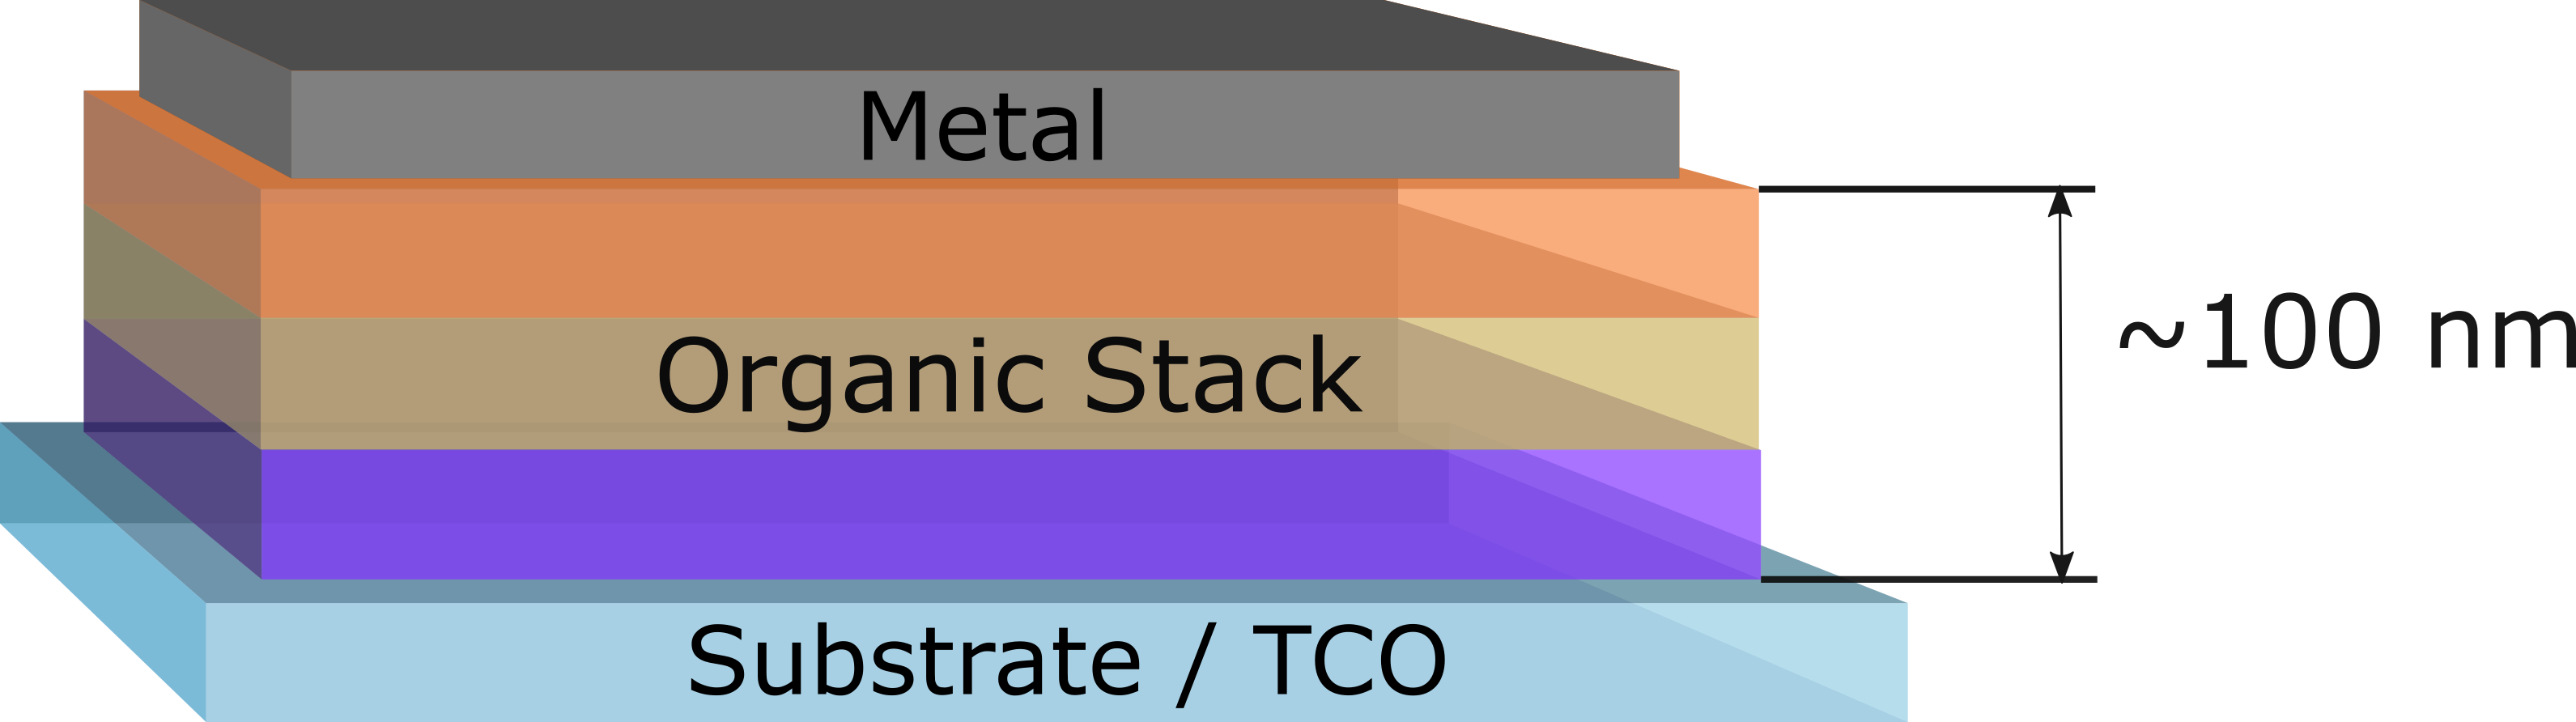
\includegraphics[width=.48\textwidth]{oleds/layer_diagram}
\caption{Basic layer diagram for OLED devices.}
\label{fig:oleds_layer_diagram}
\end{wrapfigure}

Organic Light-Emitting Devices (OLEDs) consist of an organic layer stack sandwiched between two electrodes.
For light to escape, one of the electrodes is transparent, and in most lab scale devices, this is the bottom contact.
This is often accomplished by using glass coated with Indium Tin Oxide (ITO) as a transparent conducting material.
The opposing contact is typically a metal, and in most cases Aluminum.
An example of this type of structure is shown in Figure \ref{fig:oleds_layer_diagram}.

The organic stack of devices is typically 80 nm or more and consists of multiple layers.
For most materials, deposition from the vapor phase at rates of ~1 \r{A}/s does not provide the time or energy needed to rearrange into a crystal, and thus yields amorphous films, showing minimal short and medium range order.\supercite{Tao2011,Shirota2007,Kafer2005,Maldonis2017,Maldonis2015,Zhang2017,Zhang2016a}
However, most materials will crystallize rapidly with annealing,\supercite{Fielitz2016} or slowly over time.\supercite{Scholz2015}

Detailed device operation will be expanded upon in Chapter \ref{sec:unified}, but the goal of the layer stack is to efficiently form and recombine excitons.
When voltage is applied, electrons are injected from the metal contact into the electron transport layer (ETL) and holes are injected from the ITO into the hole transport layer (HTL).
Carriers transport through these layers to a region where exciton formation is designed to occur.  
This can be done in a variety of ways and is discussed in detail in Section \ref{sec:oled_history}, but most modern devices use a structure with a dedicated emissive layer (EML), as shown in Figure \ref{fig:oleds_energy_level_diagram}.
In this type of device, the emitter molecule or guest, is doped at low concentration within a host matrix.\supercite{Baldo2000}
This composite film structure is used because most emissive molecules show a reduction in \pl with increasing concentration.\supercite{Turro1991a}
The host molecule is used to help transport charge to the emissive molecule and separate the guest molecules.
The host molecule is designed to have a wider energy gap, making it energetically favorable for excitons to form on the guest molecule.

\begin{figure}[ht]
\centering
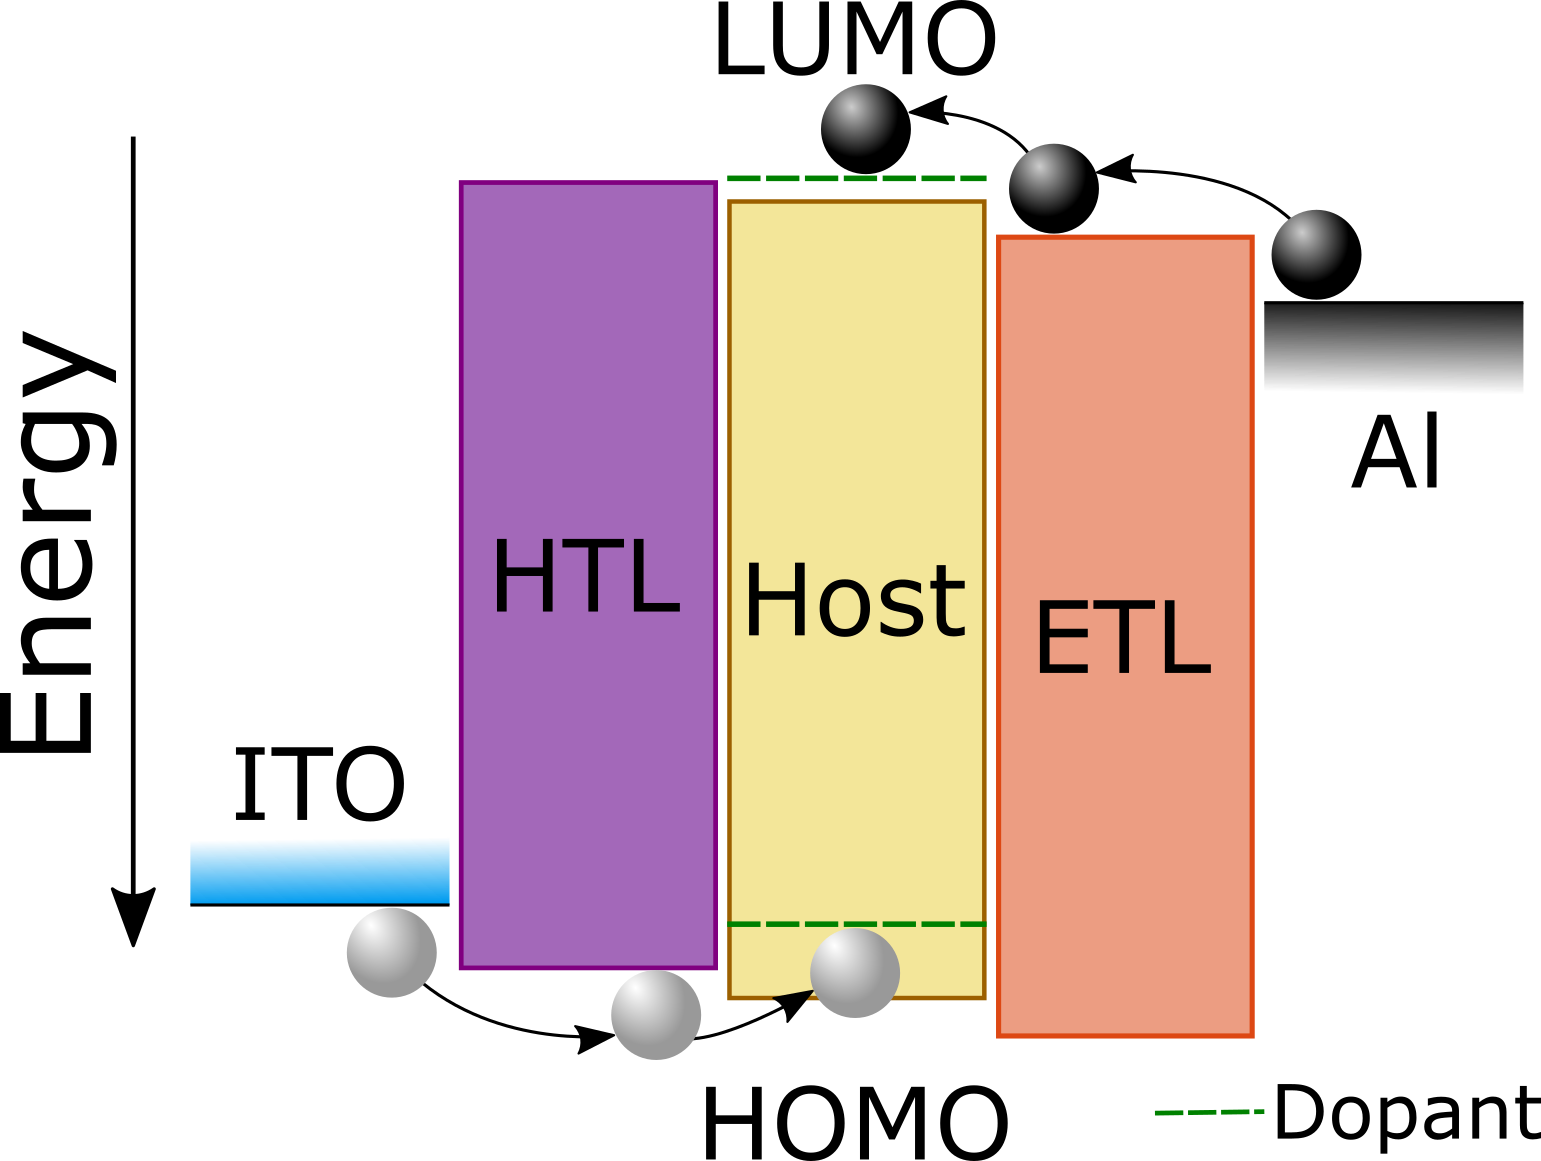
\includegraphics[width=.8\textwidth]{oleds/energy_diagram}
\caption{Energy level diagram of an OLED.  Energy is shown in reference to the vacuum level.  Electrons are shown in black spheres, holes shown in white.}
\label{fig:oleds_energy_level_diagram}
\end{figure}

The structure shown in Figure \ref{fig:oleds_energy_level_diagram} is greatly simplified from most devices.
Injection layers (HIL/EIL) are often used to aid in charge injection into the device between the electrode and transport materials.
These materials will sit energetically between the electrode and the transport layer.
To confine charges within the EML, blocking layers (HBL/EBL) are often used between the EML and the opposing transport layer.
For example, a hole blocking layer would sit between the EML and the ETL and would have an energy level similar to the ETL, so electron transport would not be disrupted, but would have a high HOMO energy or a low hole mobility.
These types of layers are often added as needed based on the energetic levels of the other materials in use.

\subsection{Efficiency Components}

\begin{figure}[ht]
\centering
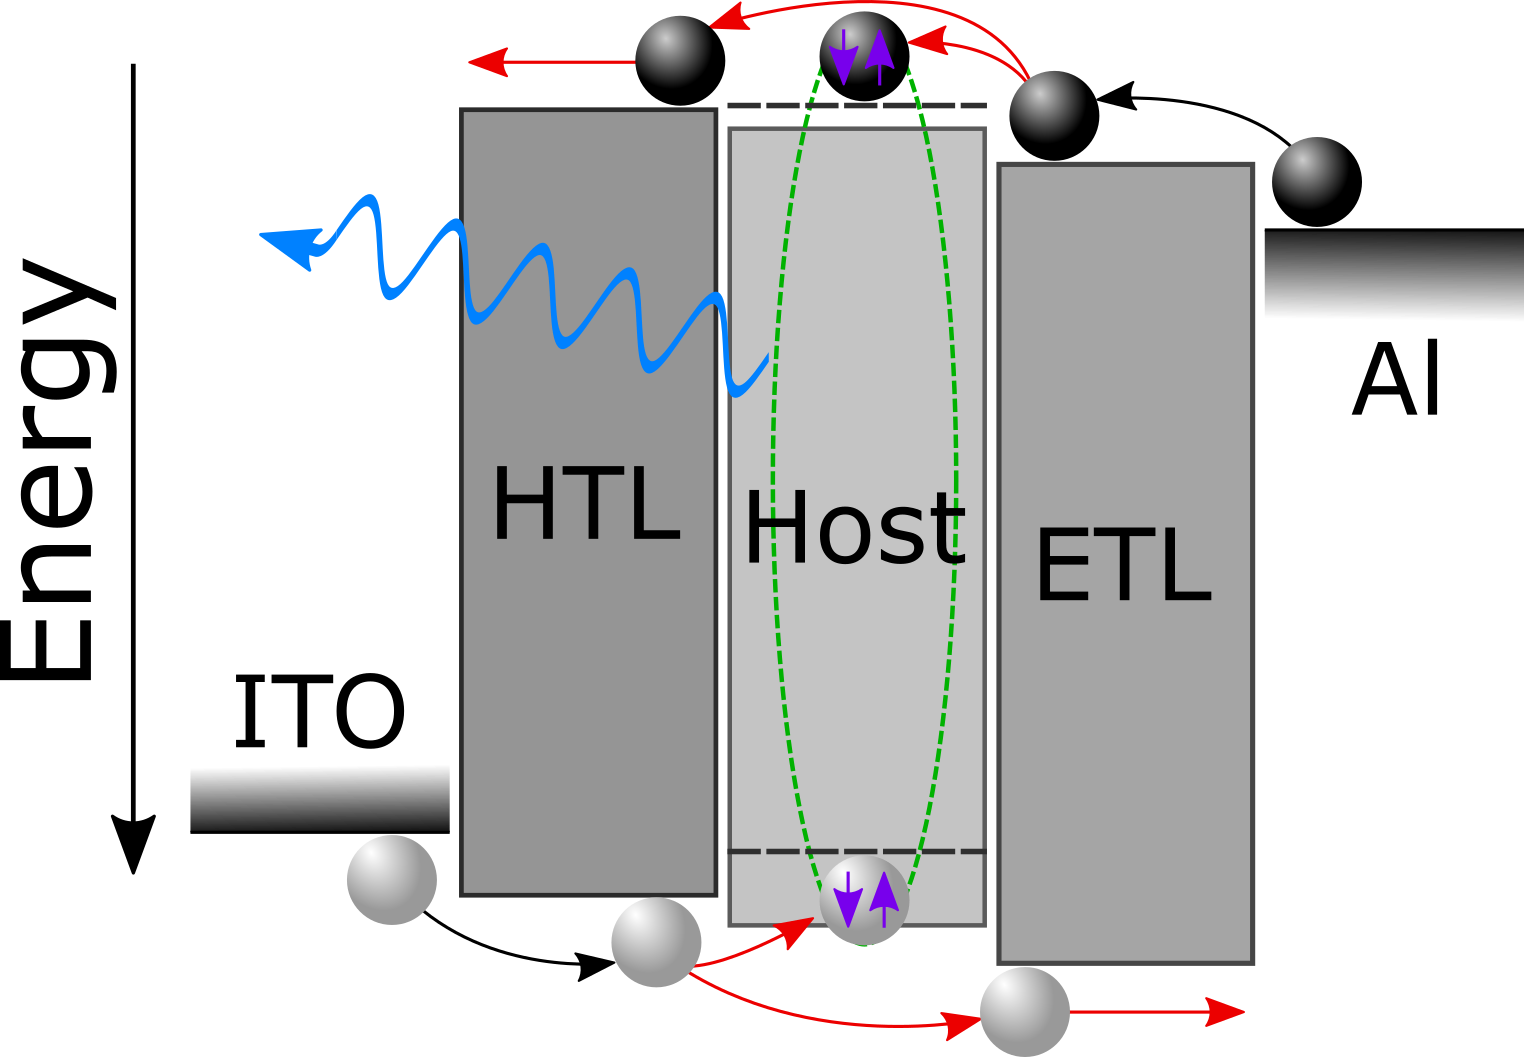
\includegraphics[width=.8\textwidth]{oleds/energy_diagram_EQE}
\caption{External Quantum Efficiency on energy level diagram.  \oc represented in blue, \pl in green, $\chi$ in purple, and \ef in red.}
\label{fig:oleds_energy_level_diagram_EQE}
\end{figure}

Device efficiency is often thought of as a four component process as:\supercite{Baldo1998a}

\begin{equation}
\eqe=\chi\pl\ef\oc
\label{eqn:eqe}
\end{equation}

The efficiency with which injected charges form excitons is the exciton formation efficiency, \ef (traditionally called charge balance,$\gamma$).
This is competitive with charge loss through the device and is shown in red in Figure \ref{fig:oleds_energy_level_diagram_EQE}.
In modern devices, \ef can approach 100\% at the maximum efficiency point.
Electrically, excitons are formed in a 3:1 Triplet:Singlet ratio, as discussed in Chapter \ref{sec:excitons}.
The radiative spin fraction, $\chi$, captures the fraction of these formed excitons that are able to emit.
For fluorescent materials, $\chi=1/4$ and for phosphorescent materials, $\chi=1$.
The photoluminescence efficiency, \pl is the efficiency of photon generation from the radiatively allowed excitons and can reach 100\%
The out-coupling efficiency, \oc, is the fraction of photons that escape the device in the forward viewing direction, and is competitive with wave-guided modes and surface plasmons.\supercite{Furno2010,Furno2012}
For most devices \oc is the limiting process for efficiency, and typically is limited to 20-30\%, but can be aided by enhancing films or layers.


\section{Fabrication Processes}\label{sec:oleds_fabrication}

Substrates consist of glass pre-coated with indium-tin oxide (ITO).  
Prior to deposition, substrates are cleaned using 5 minutes each of sonicated Tergitol, water, and two cycles of acetone, followed by two cycles of boiling isopropanol.  
This is followed by a UV-ozone treatment for 10 minutes.  
Large area devices on patterned ITO are spin coated with a solution processed hole conducting planarizing layer.
In my time in the group, this started with Pedot-PSS and has transitioned to the more commercially used Plexcore AQ-1200.
Pedot-PSS is water based and seemed more susceptible to treatment conditions prior to deposition, such as freezing.
AQ-1200 has been a more reliable material.
AQ-1200 has been replaced with AQ-1250, which appears to be the same formula, but with tighter control over consistency.
For all solution processed layers, spin coating is done for 30 seconds at 3000 rpm, followed by a 30 minute bake at 150 $^\circ$C.

\begin{figure}[ht]
    \centering
    \begin{subfigure}{.3\textwidth}
    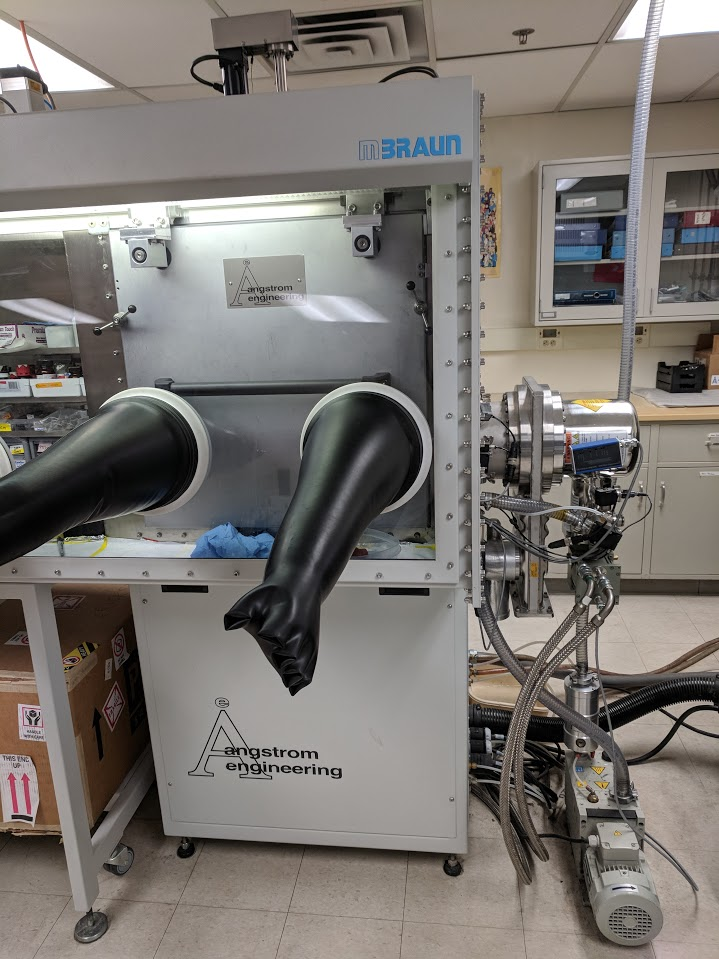
\includegraphics[width=\textwidth]{oleds/chamber}
    \caption{}
    \label{fig:oleds_angstrom}\par\vfill
    \end{subfigure}
    \begin{subfigure}{.3\textwidth}
    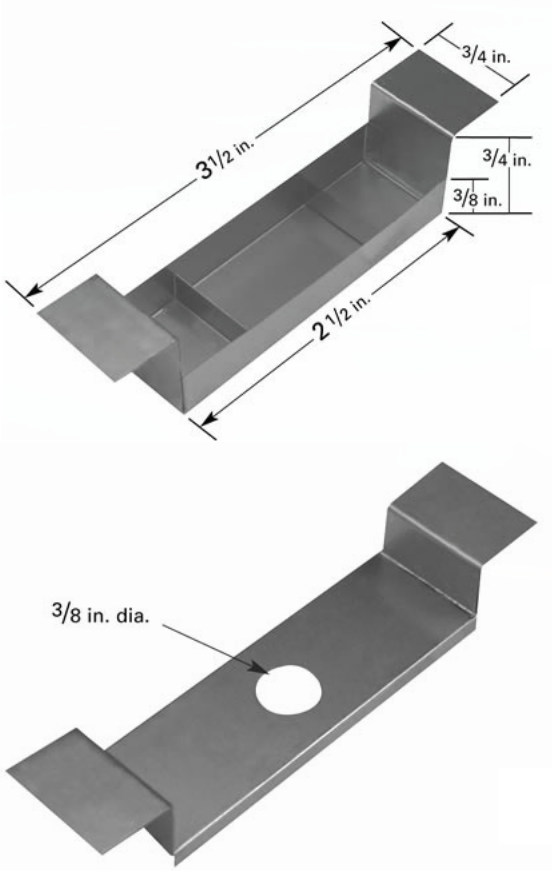
\includegraphics[width=\textwidth]{oleds/dep_boat}
    \caption{}
    \label{fig:oleds_deposition_boat}
    \end{subfigure}
    \begin{subfigure}{.3\textwidth}
    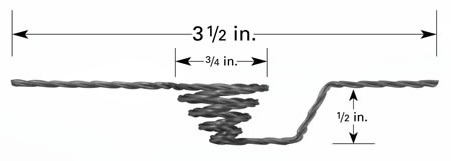
\includegraphics[width=\textwidth]{oleds/al_boat}
    \caption{}
    \label{fig:oleds_al_boat}
    \end{subfigure}
\caption{a. Angstrom vacuum chamber b. Organic deposition boat c. Aluminum deposition boat}
\end{figure}

Within our lab, the standard fabrication process for OLEDs is thermal evaporation at base pressures <10$^{-7}$ Torr.  
This is done in an Angstrom Engineering vacuum deposition chamber from tungsten boat sources for organic materials, shown in Figures \ref{fig:oleds_angstrom} and \ref{fig:oleds_deposition_boat}, respectively.
Material deposition rates can be measured using quartz crystal monitors (QCMs) during deposition.
The absolute rate of material deposition can be calibrated by conducting ellipsometry on grown films to determine thickness.
This chamber allows simultaneous deposition of up to 4 materials at a time.
Co-deposition of materials allows for the creation of doped layers, which can even be varied with time to create graded composition profiles.
For most devices, cathodes consist of 1 nm of lithium fluoride, from a dimple boat, followed by 100 nm of Aluminum, from the boat shown in Figure \ref{fig:oleds_al_boat}.

For unpatterned devices, the whole substrate is coated in ITO, and device pixels are formed using a metal mask that defines the device area.
In this case, to contact devices, contact must be made with the ITO for the anode and the Al cathode.
A hard metal probe is used to contact the ITO by poking through the organic stack.
However, the metal must be contacted without damaging the metal or underlying organic stack, as any damage would disrupt the device behavior, and at worst, short the contact to the ITO anode.
In order to contact the metal, a 100$\mu$ gold wire is used to gently contact the metal surface.

\begin{figure}[ht]
    \centering
    \includegraphics[width=.7\textwidth]{oleds/masks}
    \caption{a. ITO Pattern b. Organic Mask c. Metal Mask d. Mask Overlays.  Device area shown in red.}
    \label{fig:oleds_masking}\par\vfill
\end{figure}

Patterned devices consist of a patterned ITO substrate with a corresponding patterned metal mask, where the intersection forms the device area.
To ease contacting, an ITO pad is typically placed below the metal at the contact point outside of the organic deposition region as demonstrated in Figure \ref{fig:oleds_masking}.
This method allows for contacting the device off of the device active area, and does not suffer from the difficulty of contacting and is essential for devices to be encapsulated.
In this case, it is important to consider lateral transport within the HIL.
A sharp edge on the ITO pattern can result in a discontinuity of the organic stack at the device edges and can frequently short the device with metal directly in contact with the ITO.
To prevent this, a planarizing layer is used which minimizes the effects of ITO roughness and the discontinuity of the step edge.
While this is effective, planarizing layers are designed to have high mobility and lateral conduction could become important as it may lead to shorting between the anode and cathode ITO pads.
To prevent this in our devices, the planarizing layer is disturbed between the two pads in order to disrupt lateral transport.

For device lifetimes, to minimize oxygen exposure, devices are packaged.
This is done before devices are exposed to oxygen levels outside of a glovebox.
A UV cured epoxy seal is formed around the device active area and is capped with a glass microscope slide cover slip.
The epoxy is then cured with 3 minutes of exposure to a UV lamp.
For extreme long lived devices or higher shelf life, a desiccant can be used, but this is not common in our lab due to the relatively short lifetimes that we are studying.


\section{Characterization}

Though numerous characterizations exist to analyze devices, the standard metrics of performance consist of current-voltage, luminance, and efficiency.
Luminance is typically calculated in candelas per meter squared ($cd/m^2$).
There are three common efficiency metrics for devices, including the external quantum efficiency (\%), the power efficiency ($W/W$) and the luminance efficiency (lm/W).
Though dependent on field of study, for academic OLED interests, the most commonly explored metric is the external quantum efficiency (\eqe).

\subsection{Current Voltage and Luminance}

\begin{wrapfigure}{r}{.5\textwidth}
    \centering
    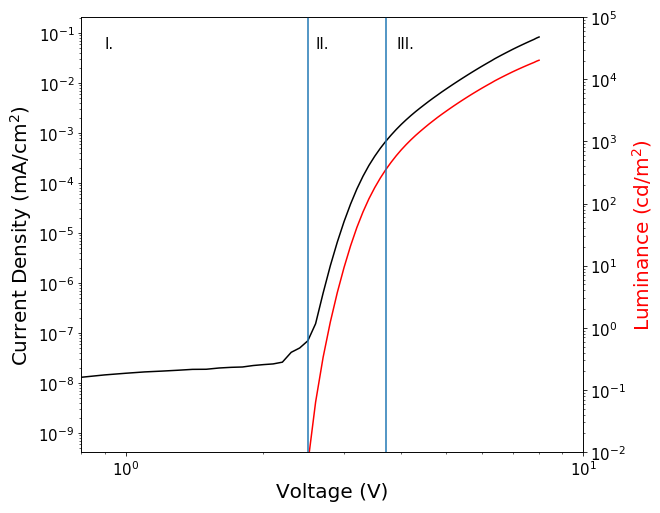
\includegraphics[width=.48\textwidth]{oleds/ivl}
    \caption{a. Device current voltage  and luminance voltage behavior}
    \label{fig:oleds_ivl}\par\vfill
\end{wrapfigure}

The current-voltage behavior of most OLEDs follows a diode-like current-voltage dependence.
This is characterized by a weak dependence of current on voltage below some threshold, followed by a strong dependence at high voltage, as shown in Figure \ref{fig:oleds_ivl}.
In terms of device operation, at low voltage below turn-on (Region I), carriers do not have enough energy to make the transitions between molecular orbital energy levels and cannot be injected into the device.
Soon after turn on, carriers are overcoming the injection barriers of the material stack and in an ideal device, forming a strong recombination current for light emission (Region II).
In this region, the current is limited by carrier injection and follows an exponential dependence as carriers overcome the injection barrier potential.\supercite{Pope1999}
At high voltage, injection barriers have been overcome and there is a charge buildup in the device which limits the current.
This region is known as the space-charge limit and the current-voltage characteristic shows a power law dependence.\supercite{Pope1999,Mark1962,Lampert2002a}
In a well formed device, luminance should closely follow current, as most current should be going to recombination and exciton formation.

For device brightness characterization, either optical power or luminance can be used.
Optical power is simply a characterization of the total photon power exiting a device.
This is typically calculated by measuring the total device light output using a large area photodiode.
For optical power or optical power density measurements, it is important to know the measured light producing region being measured.
This can either be done by ensuring the total device area and all light output is measured, in which case the area of interest is the device area, or by measuring a known subsection of the device.
The current output by the detector can be related to the incident optical power by the responsivity function of the detector, reported as a function of wavelength as $W/A$.
A typical responsivity for a silicon detector is shown in Figure \ref{fig:oleds_responsivity}a.

\begin{wrapfigure}{r}{.5\textwidth}
    \centering
    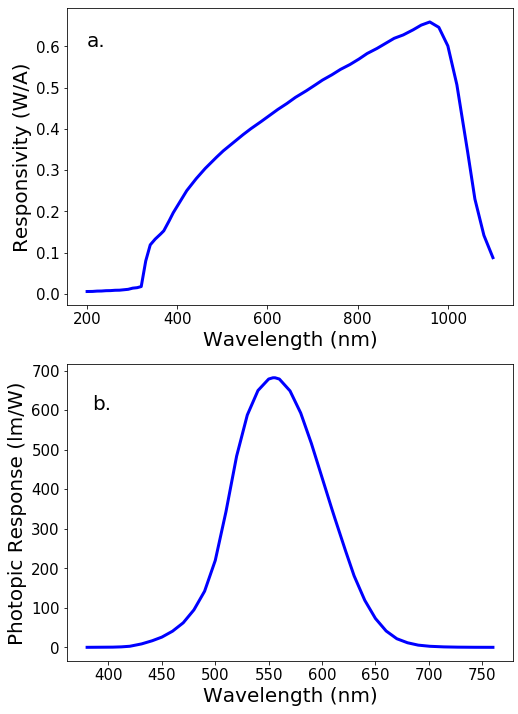
\includegraphics[width=.48\textwidth]{oleds/responsivity}
\caption{a. Silicon detector responsivity b. Photopic response}
\label{fig:oleds_responsivity}
\end{wrapfigure}


Luminance is reported in candelas per meter squared ($cd/m^2$), sometimes called a 'nit'.
The candela is a measure of perceived light intensity per solid angle and is equivalent to 1 candle power.
To measure luminance, the light output must be normalized to the wavelength dependent response of the human eye, known as the photopic response, shown in Figure \ref{fig:oleds_responsivity}b.
This is typically done in one of two ways.
The first method (employed by our group) is to use a spectrometer to measure the output light spectrum in Watts per nanometer.  
Then the spectrally averaged photopic response can be found for the light source of interest.
Then, the output optical power can be measured by a simple photodiode and calibrated using the average photopic response.
Alternatively, a photodiode can be filtered and modified so that the responsivity function matches the photopic response.
In this case, the photodiode would directly output the luminance.
Both methods are standardly used in research groups.\supercite{Hershey2016,Inoue2016,Forrest2003}


\subsection{Efficiency}\label{sec:efficiency_analysis}

As mentioned previously, there are three common measures of device efficiency.  
The first is power efficiency, measured in $W/W$.
This is straight forward to calculate given the previous discussion of measuring optical power.
The luminance efficiency $lm/w$ is related to the luminance output.
The lumen is a measure of total light output and is related to the candela by 1 lm = $2\pi$ candelas.
A keen eye would note that the candela is normalized per solid angle and a factor of $4\pi$ may be expected, but OLEDs are only able to emit in the forward direction.

The external quantum efficiency (\eqe) is a measure of photons exiting the device per electron injected.
The photon flux out of the device can be calculated from the optical power by dividing by the average photon power, $hf_{avg}$, where $f_{avg}$ can be calculated from the measured spectrum.
The injected electron flux is simply $I/q$ where $I$ is the device current.
The mathematical details of this model are discussed in detail by \textcite{Forrest2003}.%\supercite{Forrest2003}

\subsection{Chromaticity}
\begin{figure}[ht]
\centering
\begin{subfigure}{.4\textwidth}
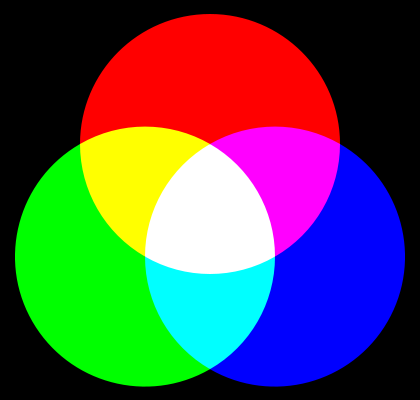
\includegraphics[width=\textwidth]{oleds/color_addition}
\caption{}
\label{fig:oleds_color_addition}
\end{subfigure}
\begin{subfigure}{.4\textwidth}
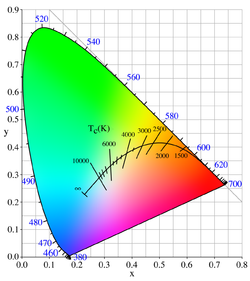
\includegraphics[width=\textwidth]{oleds/chromaticity}
\caption{}
\label{fig:oleds_cie}
\end{subfigure}
\caption{a. Simple color addition diagram. b. CIE $xyY$ color space.}
\end{figure}
In addition to the efficiency and brightness characterization, the quality of light can also be assessed, known as chromaticity.
This is very important for both displays and lighting applications.
This characterization is standardly done using the CIE chromaticity diagram and xyY color space.\supercite{Smith1931,Wright1929,Guild1932}

The chromaticity of an emitter is defined to reflect the sensitivity of the human eye.
In the eye, there are two color sensing cones, roughly corresponding to red, green, and blue.
The wavelength sensitivity of these cones for red, green, and blue are defined as $\bar{x}(\lambda)$,$\bar{y}(\lambda)$, and $\bar{z}(\lambda)$, respectively.
A three dimensional color-space is then defined to define any color using

\begin{equation}
A=\int_\lambda L_{e,\Omega,\lambda}(\lambda)\bar{a}(\lambda)d\lambda
\label{oleds_tristimulus}
\end{equation}

where $A$ and $\bar{a}$ are $X,Y,Z$ and $\bar{x},\bar{y},\bar{z}$.
These three dimensional coordinates are able to accurately describe the light, but are not very useful for visualizing the color-space.
Therefore, the brightness is normalized out, leaving us with two color coordinates and a brightness value.
Since our eye is most sensitive to green stimulus, the $Y$ coordinate is taken to represent the brightness.
The color coordinates can be normalized by

\begin{equation}
a=\frac{A}{X+Y+Z}
\label{oleds_color_coordinates}
\end{equation}

where $a$ and $A$ are $x,y,z$ and $X,Y,Z$.
Note that $x$ is a new color coordinate, not the standard observer sensitivity, $\bar{x}$.
This remapping still has three coordinates, but here, $z=1-x-y$.
Therefore, the color can be represented using just $x,y$.
This can be seen in Figure \ref{fig:oleds_cie}, where the perimeter is defined by mapping single wavelength light through these coordinate transformations.
All possible visible colors are defined within the locus, and $x,y$ coordinates are shown on the axes.
For white light, the color temperature is calculated in reference to a black-body emission and is also shown in Figure \ref{fig:oleds_cie}.
While sophisticated in calculation, it is important to note that this concept of color-space is simply an extension of the color addition shown in Figure \ref{fig:oleds_color_addition}.

\subsubsection{RGB}
\begin{wrapfigure}{r}{.5\textwidth}
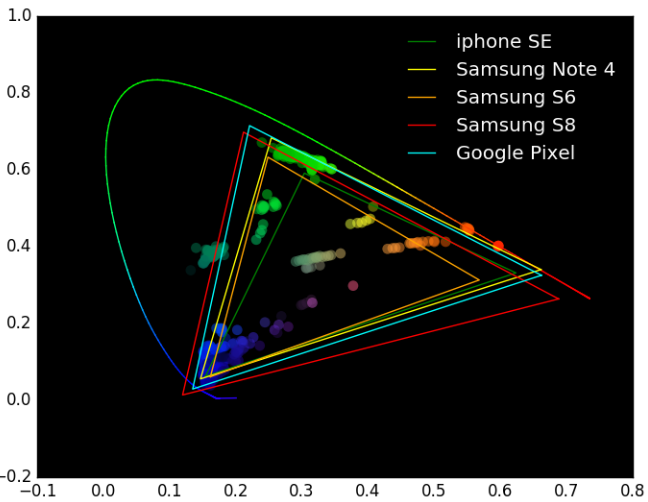
\includegraphics[width=.48\textwidth]{oleds/cie_phones}
\caption{Various phone display limits shown on CIE coordinates}
\label{fig:oleds_cie_phone}
\end{wrapfigure}

For display applications, a single red, green and blue emitter are used, each of which will have $x,y$ coordinates which can be expressed on the CIE diagram.
Using this method, only colors within the enclosed triangle can be expressed, making it critical for a vibrant display to maximize the area of this triangle.
Various phone displays are shown in Figure \ref{fig:oleds_cie_phone}, with the pure color components being generated using a RGB color picker application.
Interestingly, the iPhone SE, the only phone not using an OLED display, shows the worst response in the green, a clear advantage of OLED color representation.
The scatter points in this figure represent individual pixels measured in the course of this thesis.

One limit of RGB color representation is that it is not consistent across displays.
For example, the RGB coordinate (0,1,0) looks different on the Google Pixel versus the iPhone SE due to their different CIE coordinates.
To account for this, display RGB values can be calibrated to accurately represent the CIE coordinates.
However, in doing so, the color space available to the display is shrunk and the full color range of the display cannot be used.
This is an important issue in commercial devices where consumer demands must be carefully considered with respect to the trade off between accurate and vibrant colors.
This trade off was clearly seen in the release of the Google Pixel 2, where consumers complained about dull colors because the manufacturers used a calibrated color space.\supercite{Bohn2017}

\section{Historical Development}\label{sec:oled_history}
\subsection{The First OLEDs}

\begin{wrapfigure}{r}{.5\textwidth}
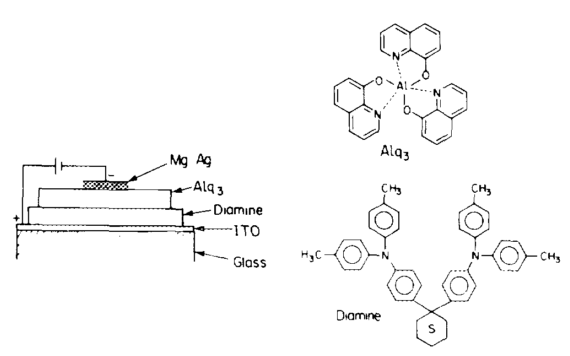
\includegraphics[width=.48\textwidth]{oleds/tang}
\caption{Structure of the first OLED cell from \textcite{Tang1987}.  Diamine is commonly referred to now as TAPC.}
\label{fig:oleds_tang}
\end{wrapfigure}

Early interest in organic materials was generated based on use for organic laser dyes and the high fluorescence efficiency demonstrated.\supercite{Venkataraman1971,Schafer1977,Dresner1969}
Early attempts at producing electroluminescent devices tried contacting organic crystals, but required extremely high voltages to produce any light.\supercite{Williams1970,Helfrich1965}
The first successful OLED was demonstrated by \textcite{Tang1987} in 1987, one of the first to utilize vacuum deposition for thin films.
This was a bilayer device, with the structure shown in Figure \ref{fig:oleds_tang}, using TAPC at 75 nm thick and Alq$_3$ 60 nm, responsible for the emission of the device, centered around 550 nm.
These devices achieved \eqe $\approx$1\% and showed rapid degradation.

In fluorescent cells, $\chi=0.25$ and without out-coupling enhancement $\oc \approx 0.20$, leaving a maximum \eqe of just 5\%.
Doped films were investigated soon after these initial findings in order to capitalize on the improved \pl at low concentration.\supercite{Tang1989a}
This host with emissive guest system is utilized by almost all devices.


\subsection{Phosphorescence}
OLEDs saw a massive improvement in possible efficiency in 1998 with the introduction of phosphorescent dyes.\supercite{Baldo1998a}
These dyes use a heavy metal atom to create a metal-ligand charge transfer state, which allows mixing of the singlet and triplet states, and thus emission from the triplet exciton.
With all excitons able to emit, including the triplet state, the internal quantum efficiency ($\eta_{IQE}$) raises to 100\%.
These devices utilized the red phosphor PtOEP in conjunction with the laser dye DCM2.
This work comments on quenching at high current of the phosphor, a continuing problem which will be discussed further in Section \ref{sec:oleds_roll_off}.\supercite{Reineke2007,Hershey2016}
Pure red and green emission devices utilizing only a phosphorescent dopant were developed soon after, along with the development of the ubiquitous green emitter, Tris[2-phenylpyridinato-C$^2$,N]iridium(III) (Ir(ppy)$_3$), shown in Figure \ref{fig:oleds_irppy}.\supercite{OBrien1999a,Adachi2000}

\begin{wrapfigure}{r}{.4\textwidth}
\centering
%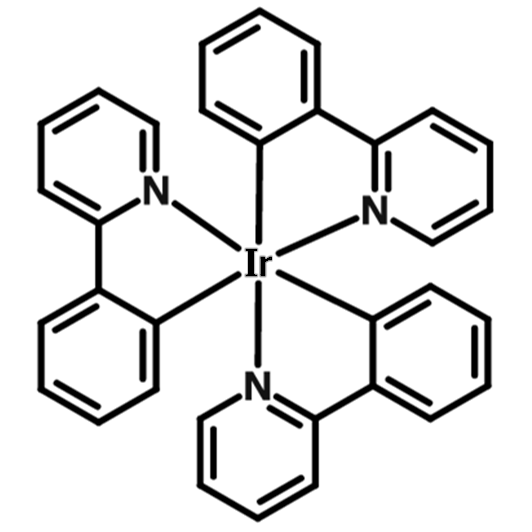
\includegraphics[width=.38\textwidth]{oleds/irppy3}
\setatomsep{2em}\chemfig[][scale=1.0]{Ir?(-[:60,2]*6(-(-*6(=N?-=-=-))=-=-=))(-[:180,2]*6(-(-*6(=N?-=-=-))=-=-=))(-[:300,2]*6(-(-*6(=N?-=-=-))=-=-=))}
\caption{Molecular structure of the green phosphor, \irppy}
\label{fig:oleds_irppy}
\end{wrapfigure}

Since the realization of the phosphorescent OLED, internal quantum efficiencies nearing 100\% for green, red, blue, and white devices have been demonstrated.\supercite{Su2008a,Erickson2010}
With high efficiency achieved, attention has shifted to maximizing lifetimes.\supercite{Scholz2008}
Despite the high efficiency of blue phosphorescent devices, lifetimes still remain limiting and blue fluorescent materials are still used in commercial technologies.


\subsection{Thermally Activated Delayed Fluorescence}

\begin{wrapfigure}{r}{.5\textwidth}
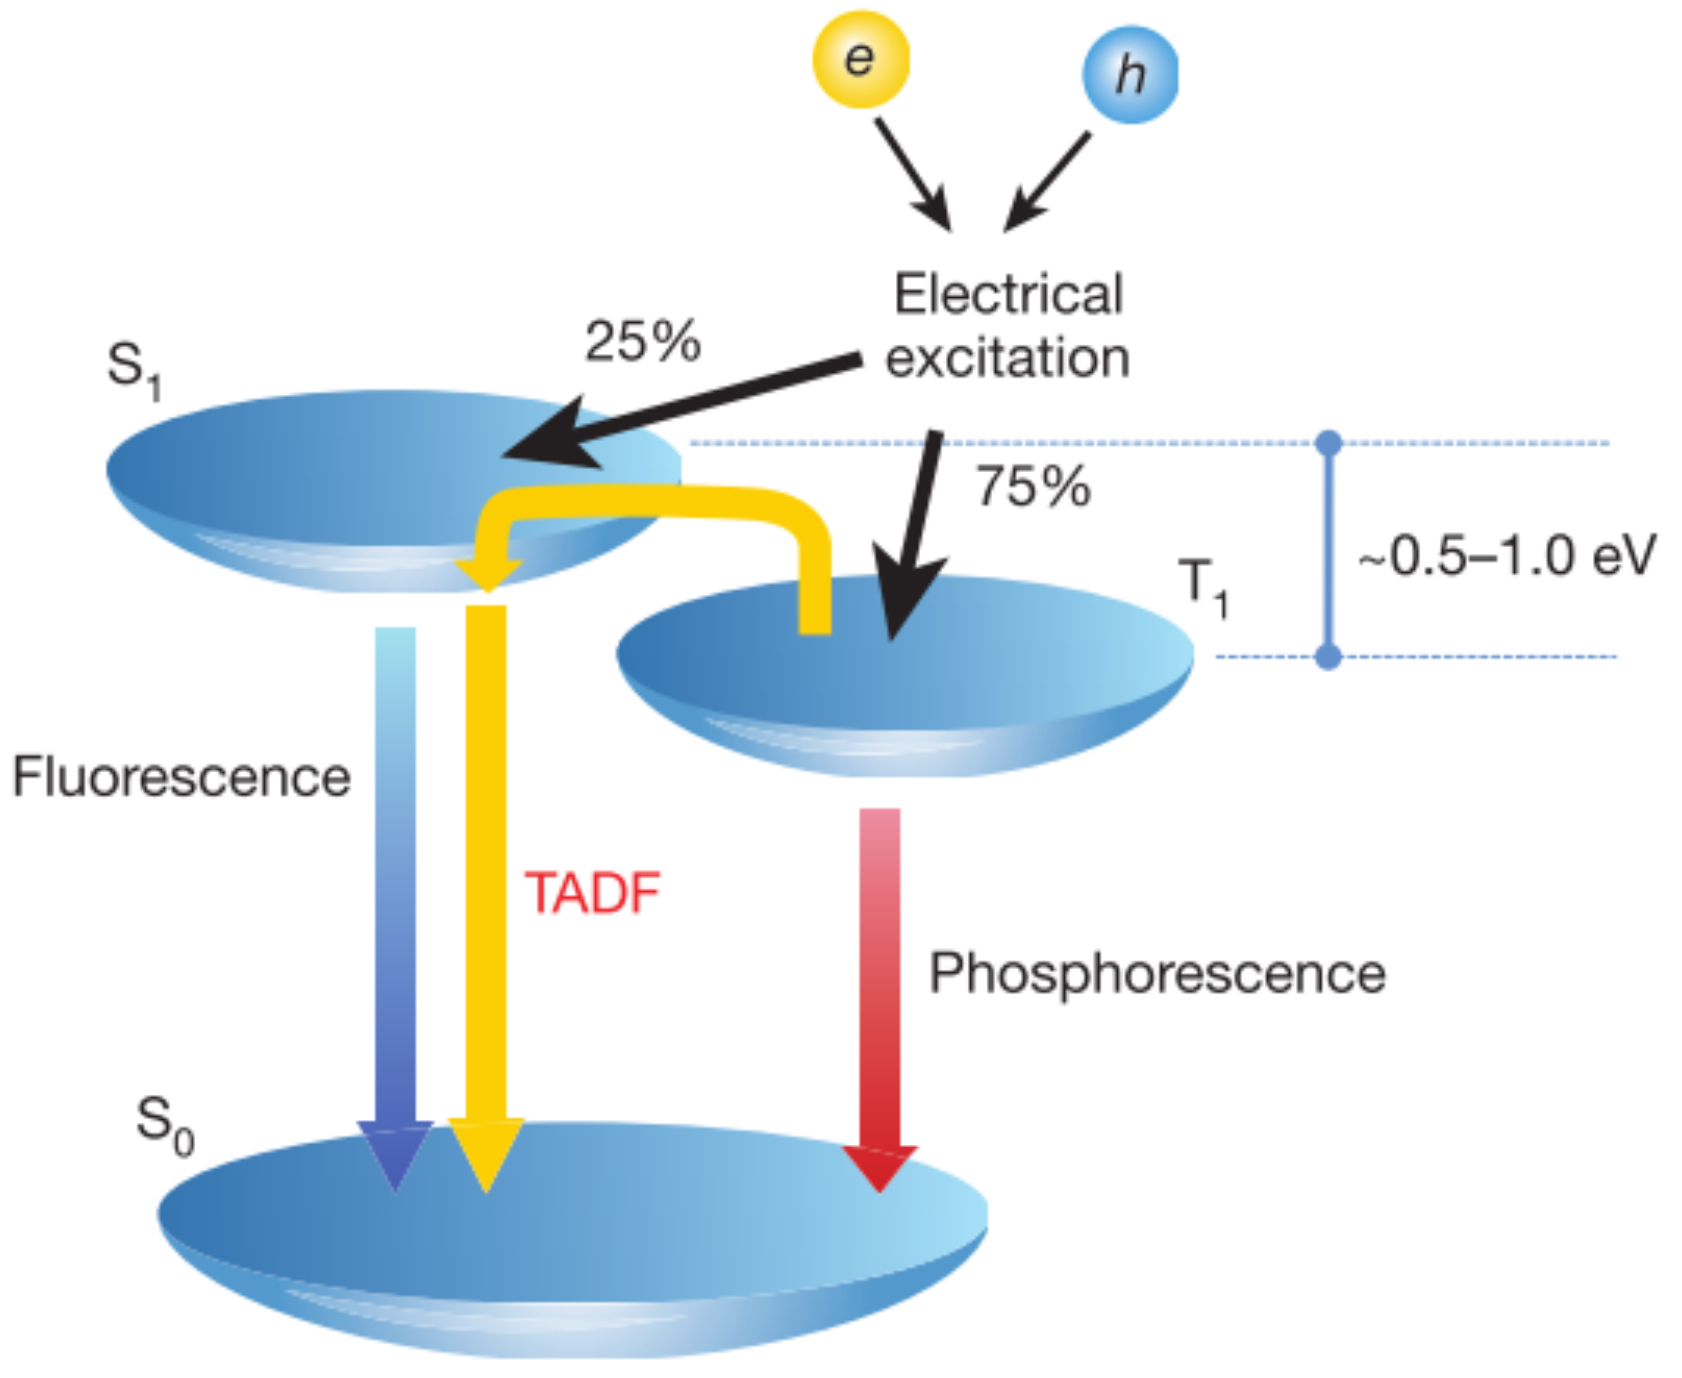
\includegraphics[width=.48\textwidth]{oleds/tadf}
\caption{Reverse intersystem crossing for TADF materials.  Figure taken from \textcite{Uoyama2012}.}
\label{fig:oleds_tadf}
\end{wrapfigure}

While phosphorescent devices have been able to demonstrate high efficiency necessary for commercialization, this has come at a cost.
Namely, in the use of expensive and rare heavy metal atoms, such as Ir(III), Pt(III), and Os(II).\supercite{Adachi2001b}
In order to utilize the triplet excitons, reverse intersystem crossing is utilized.
Chapter \ref{sec:excitons} and Figure \ref{fig:orgSemi_jablonski} discuss intersystem crossing as an energetically favorable process as the triplet is lower energy than the singlet.
However, if molecules are designed where the singlet and triplet energies difference ($\Delta E_{ST}$) is small ($<1eV$), thermal energy can make the reverse intersystem crossing competitive with intersystem crossing ($k_{RISC}\approx k_{ISC}$).
This allows for Thermally Activated Delayed Fluorescence (TADF), shown in Figure \ref{fig:oleds_tadf}.\supercite{Zhang2012b,Zhang2014a,Uoyama2012}
TADF materials are a rapidly developing technology that has shown many benefits for efficiency, and rules are being established for molecular design.\supercite{Menke2016,Inoue2016,Li2013,Wang2015,Liu2015,Kim2015,Jankus2014,Lavie-Cambot2008,Zhang2012b,Endo2009,Yersin2014,Nasu2013,Uoyama2012,Zhang2012c,Hofbeck2015,Linfoot2014,Reineke2014a,Zhang2014a}
These materials are also being investigated for benefits to device lifetime.\supercite{Mehes2014,Cho2014}


\section{Efficiency Roll-Off}\label{sec:oleds_roll_off}

In operational OLEDs, it is almost universally observed that efficiency reduces at high brightness and current density, an affect known as the efficiency roll-off,demonstrated in Figure \ref{fig:oleds_rolloff}.\supercite{Erickson2014,Song2011,Wehrmeister2015,Son2008,Murawski2013,Giebink2008c,Song2010,Xiang2016,Coehoorn2015,Reineke2009,Mezyk2005,Baldo2000a,Reineke2007,Kohler2009,Hershey2016,Erickson2013a}
This has been extensively studied and largely attributed to the bimolecular quenching processes discussed in Chapter \ref{sec:excitons}, though exciton formation efficiency (\ef) is also known to contribute at a lesser degree.
This is detrimental to commercialization as high brightness is a necessity for display and lighting applications.
The bimolecular quenching at high brightness is also detrimental to device lifetime because quenching processes produce hot excited states that release excess energy into the device, which is thought to be a key factor in molecular degradation.\supercite{Giebink2008a,Coburn2017,Lee2017}
Development of electrically pumped organic lasers has proved unsuccessful because the exciton densities required to achieve population inversion lead to excessive quenching and the inability to create stimulated emission.\supercite{Baldo2002,Baldo1998a,Holmes2007,Takenobu2008,Samuel2009,Kasemann2011}

\begin{wrapfigure}{r}{.5\textwidth}
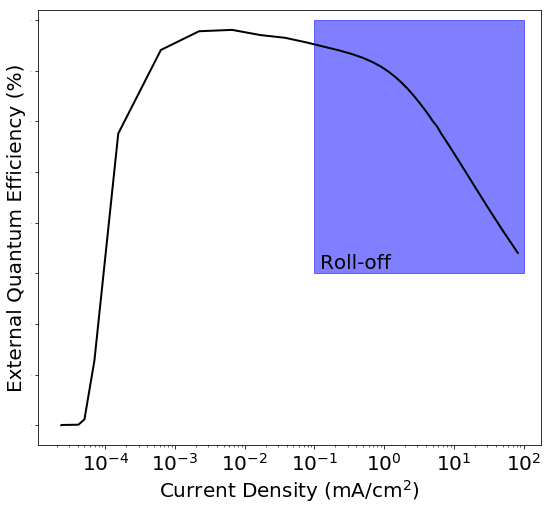
\includegraphics[width=.48\textwidth]{oleds/roll_off}
\caption{Efficiency roll-off as a function of current density}
\label{fig:oleds_rolloff}
\end{wrapfigure}

Devices are often investigated to try to reduce the roll-off, often through the broadening of the exciton recombination zone.\supercite{Wang2015,Murawski2014,Inoue2016,Soofi2017,Chopra2010,Reineke2007a,Lee2009b,Su2008a,Zang2008}
These devices have not been successful in removing the roll-off, but rather in reducing it.
Section \ref{sec:oled_operation} discussed the characterization of quantum efficiency using a four component efficiency model.  
This model fails to reproduce the roll-off behavior as it does not account for quenching.
Modeling the efficiency roll-off has been the study of numerous works and is the motivation for Chapter \ref{sec:unified}.\supercite{Reineke2007,Erickson2014,Hershey2016,Murawski2013}
These models center around a differential equations model for exciton dynamics, such as:

\begin{equation}
\frac{dn_{ex}}{dt} = - \frac{n_{ex}}{\tau}-\frac{1}{2}\ktt n_{ex}^2-\ktp n_{pol}n_{ex}+G_{ex}
\label{eqn:oleds_exciton_rate}
\end{equation}

where $n_{ex}$ is the exciton population density, $\tau$ is the exciton lifetime, \ktt is the triplet-triplet annihilation rate, \ktp is the triplet-polaron quenching rate, $n_{pol}$ is the charge density, and $G_{ex}$ is the exciton generation rate.
Here we can see that the natural lifetime is competitive with the bimolecular quenching rates, and at high exciton and charge density, the second order dependence of the quenching terms allows them to dominate.
This reduces the relative number of excitons that are decaying via the radiative rate, thus decreasing the efficiency.
These models have been successful in characterizing the rate constants and describing the roll-off behavior.
For further details, see Chapter \ref{sec:unified}.


\section{Recombination Zone Characterization}\label{sec:rz_measurement}
\begin{wrapfigure}{r}{.5\textwidth}
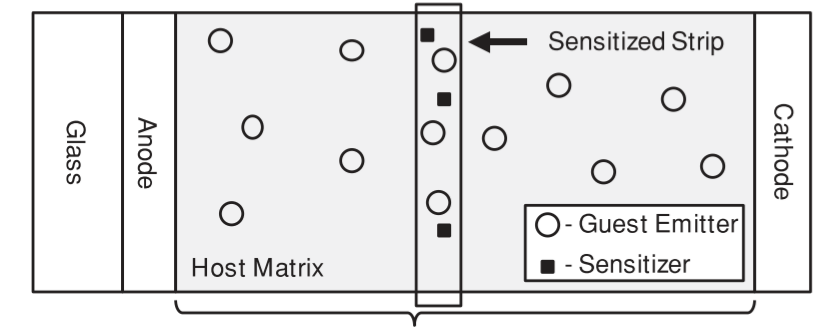
\includegraphics[width=.48\textwidth]{oleds/rz_arch}
\caption{Recombination zone measurement architecture.  The curly brace indicates the device stack.  Figure taken from \textcite{Erickson2013a}}
\label{fig:oleds_rz_arch}
\end{wrapfigure}
Both degradation and bimolecular quenching can be highly dependent on the exciton density and location, known as the exciton recombination zone (RZ).\supercite{Giebink2006,Giebink2008a,Giebink2008c,Giebink2009a,Reineke2007,Hershey2016,Hershey2017,Bangsund2018}
Therefore, it is important to be able to characterize the spatial profile of excitons.
This has been done by a variety of researchers using thin doping layers of a sensitizer molecule.\supercite{Reineke2007a,Coburn2016a,Coburn2017,Erickson2013a,Hershey2017,Bangsund2018}

In these experiments, the dopant is used to efficiently siphon excitons off of the emitter molecule and onto the sensitizer.
In order to do this, F\"{o}rster transfer to the sensitizer must be efficient, requiring significant overlap of the emitter emission and the sensitizer absorption.
\textcite{Erickson2013a} looked at the spatial extent of F\"{o}rster transfer and found that transfer was efficient within a $<4$ nm radius.
To characterize the recombination zone, sensitized layers are used and the effect of the local perturbation of the exciton density can be measured.
Translating the sensitized strip across the device as shown in Figure \ref{fig:oleds_rz_arch} allows for comparison of the relative effects and thus determination of the relative magnitude of the recombination zone.
The F\"{o}rster radius gives the maximum spatial resolution that can be obtained using this strip translation.

A quenching (non-radiative) or emissive (radiative) sensitizer can be used for these experiments.
With a quenching sensitizer, if the recombination zone overlaps with the sensitizer position, emission is lost and the efficiency is reduced.
The reduction in EL intensity can be quantified by the EL ratio of the sensitized intensity compared to the unsensitized intensity, $\beta$.
$\beta$ is directly proportional to the unquenched excitons, therefore $1-\beta$ gives the ratio of quenched excitons.

For emissive sensitizers, given the requirement of emission-absorption overlap, red sensitizers are used.
For simplicity, the sensitizer should show spectral separation of the emission from the emitter.
The intensity of the sensitizer emission is a direct measure of the local exciton density.
However, since the out-coupling is so strongly dependent on emitter position in the EML, it is essential to correct the intensity using a calculation of \oc, discussed in Chapter \ref{sec:out_coupling}.
One may note that the quenching sensitizer method should also require out-coupling correction, but since the emission is not spatially isolated, calculation of the spatially averaged out-coupling efficiency would require prior knowledge of the recombination zone shape and therefore cannot be done.
Emissive sensitizers often rely on the use of Pt(II) complexes, such as PtOEP or PtTPTBP.\supercite{Coburn2016a,Hershey2017}
Compared with Ir(III) complexes, Pt(II) shows a much longer exciton lifetime, and is therefore far more susceptible to bimolecular quenching.\supercite{Mezyk2005}
If the sensitizer is in a regime of bimolecular quenching during the measurement, a compressed version of the recombination zone will be measured.
This can be difficult to avoid at high current densities that may be of interest for measurement.

\begin{wrapfigure}{r}{.5\textwidth}
\includegraphics[width=.48\textwidth]{oleds/rz_comparison}
\caption{Recombination zone comparison for an emissive sensitizer analyzed using the quenched ratio and the emitted ratio as a function of current density.}
\label{fig:oleds_rz_comparison}
\end{wrapfigure}

An advantage of the emissive sensitizer is that the data generated can be analyzed either using the quenched ratio or using the emitted intensity.
This can be helpful for quantifying error in the method, and is demonstrated in Figure \ref{fig:oleds_rz_comparison}.
Here, we see the spatial dependence of the recombination zone for an architecture peaked at the ETL interface.
Notice that the emissive sensitizer, PtTPTBP shows a less exaggerated RZ for all current densities.  
This is likely due to bimolecular quenching on the sensitizer, which is stronger at the higher exciton densities present at the ETL interface.

When constructing these sensitizer layers, there are two popular methods.  
First, the EML can be reproduced exactly with the addition of a light doping of the sensitizer.  
This creates a strip that exactly replicates EML, but increases the difficulty of the growth, requiring one more material in a co-deposition.
An alternative is to use an extremely thin deposition of the sensitizer molecule in isolation, known as delta doping.
A deposition of 1 \r{A} is used, which since the molecular radius of the deposited material is larger than that, in reality, a discontinuous layer is produced.
When the EML is continued on top of this discontinuous layer, this is equivalent to an extremely narrow strip of a mixed layer.
This is advantageous because it make the deposition much easier and creates a very narrow strip.
However, it can be difficult to control the doping percentage as it is difficult to accurately measure films this thin.
No quantification of error on these types of doping have been reported.

In order to accurately compare the recombination zone intensity, it is essential to ensure that no differences in the transport and injection properties occur with the introduction of the sensitizer.
Since the sensitizer molecules will likely result in a trap state, it is essential to keep doping concentrations low, on the order o 1\%.
Evidence of minimal interference on the electrical properties by the sensitizer is provided by the current-voltage behavior.
If the current-voltage characteristic is within error between all of the sensitizer devices, it is often assumed that the device is representative of the control.\supercite{Erickson2013a}

\section{Single Carrier Devices}
When investigating device behavior, is often important to characterize the behavior of a single charge carrier.\supercite{Reineke2008,Reineke2007,Erickson2011}
To do this, devices have to be created that allow passage of only one carrier.
This can be accomplished by establishing energetic barriers for the opposing charge, disallowing injection, or through heavy imbalance of mobility.
\begin{figure}[ht]
\centering
\begin{subfigure}{.4\textwidth}
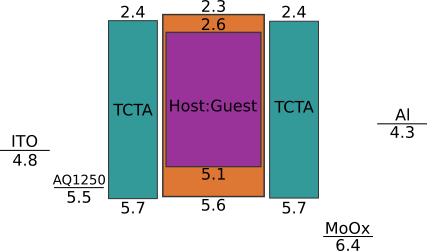
\includegraphics[width=\textwidth]{oleds/hole_only}
\caption{}
\label{fig:oleds_hole_only}
\end{subfigure}
\begin{subfigure}{.4\textwidth}
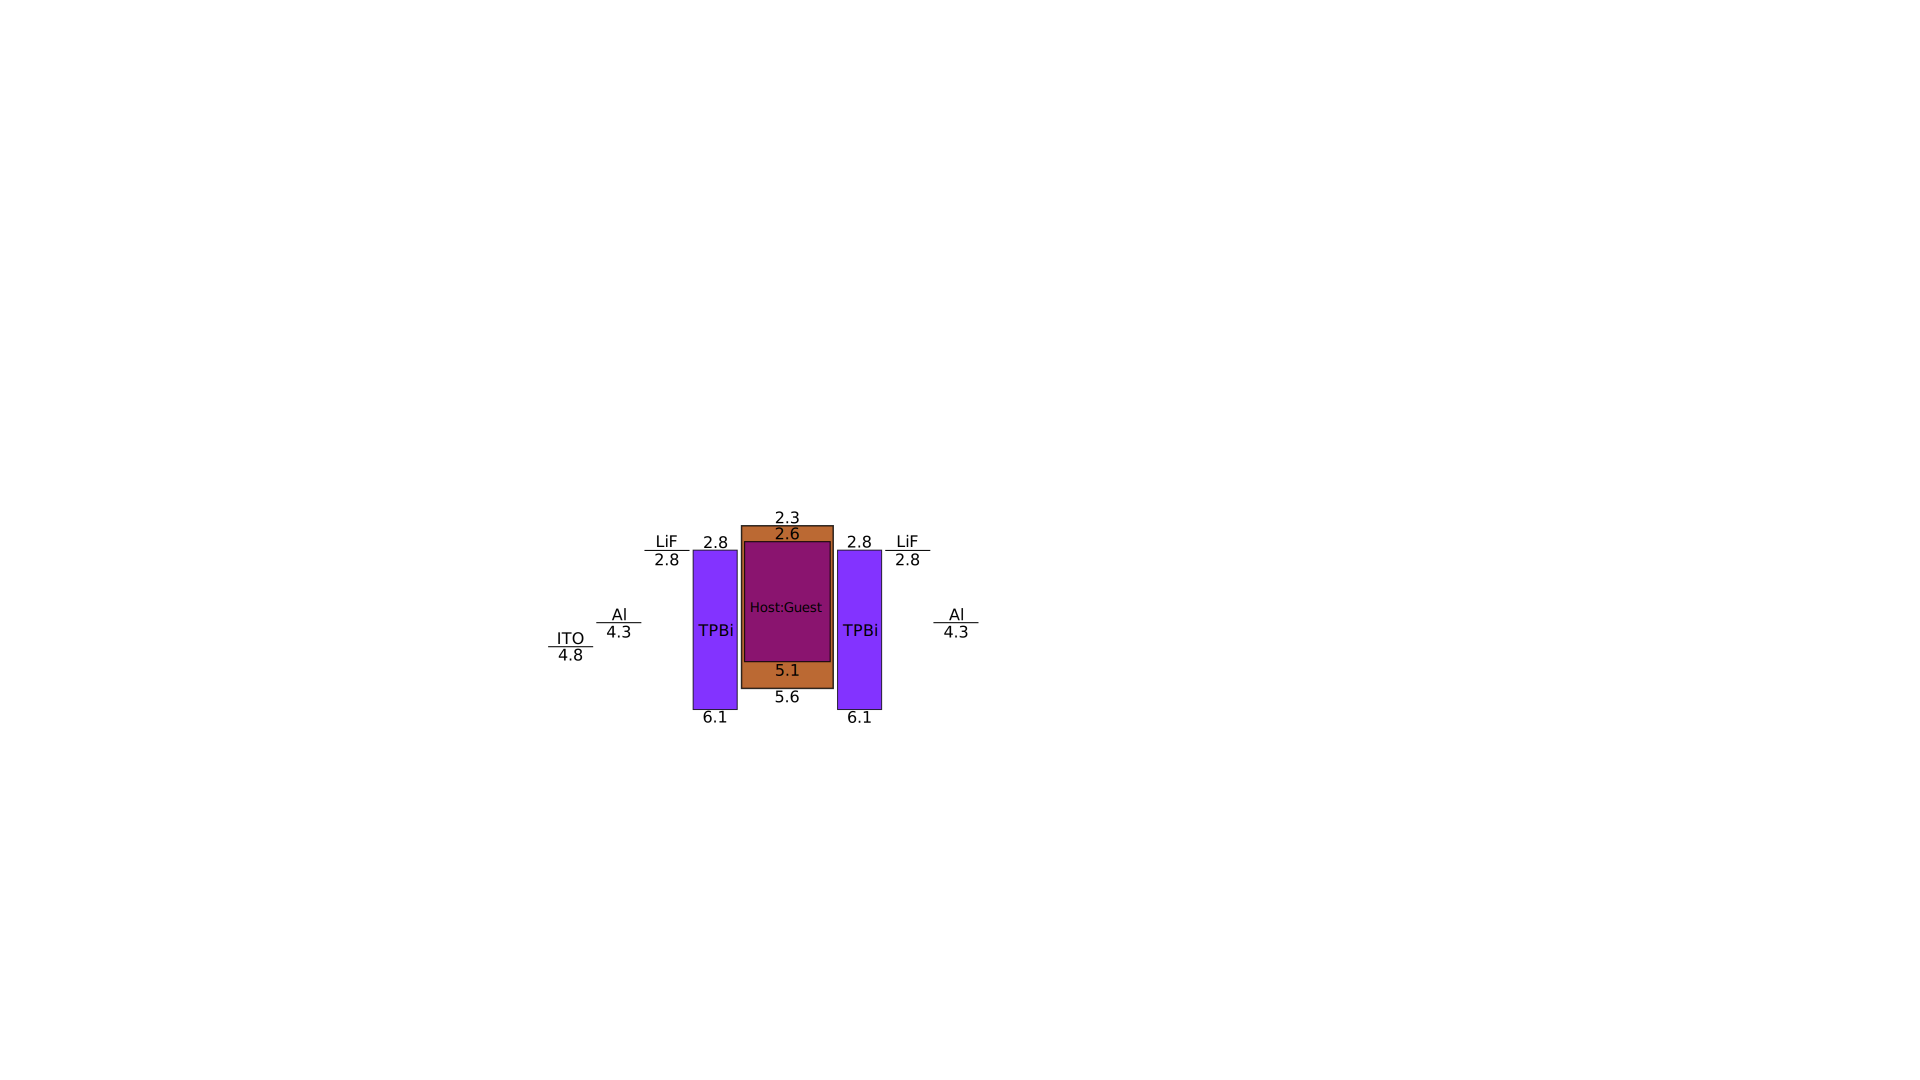
\includegraphics[width=\textwidth]{oleds/electron_only}
\caption{}
\label{fig:oleds_electron_only}
\end{subfigure}
\caption{a. Hole only device. b. Electron only device.}
\end{figure}
Examples of hole and electron only devices are shown in Figures \ref{fig:oleds_hole_only} and \ref{fig:oleds_electron_only}.
In Figure \ref{fig:oleds_hole_only}, MoO$_x$ provides a deep energy barrier for electron injection.
Additionally, TCTA is used, which has a high hole mobility and lower electron mobility, along with well aligned HOMO levels, encouraging hole transport.
In this device, positive bias is applied to the ITO contact, for no particular reason other than tradition and that it works well.
In Figure \ref{fig:oleds_electron_only}, the ITO contact does not facilitate electron injection.  
Therefore, A thin layer of aluminum is doped on top of the ITO, along with LiF, which adjusts the interface energy to more align with electrons and block holes.
TPBi is used to provide a transport barrier for holes and facilitate electrons.  
The same LiF-Al contact is used to promote electron injection.
In this device, better current-voltage characteristics are seen with positive bias applied to the ITO, in my experience.
This may be due to the properties of LiF at the ITO side interface, since in the experiments using this structure, a vacuum break occurred at that interface with LiF exposed.
We have not investigated the differences in manufacturing techniques to explore this further.

Single carrier devices have been heavily investigated and modeled for their polaron and current-voltage behavior.\supercite{Pope1999,Mark1962,Lampert2002a}
This can be used to help in analyzing these devices for dynamics and comparison to full device behavior.

\section{Operational Lifetime}
In typical lifetime characterization, devices are degraded while held at constant current density, recording the resulting luminance loss and voltage gain as a function of time.  
The lifetime is then reported as the time to reach some arbitrary fraction of the initial luminance.




\subsection{Degradation Mechanisms}\label{sec:degradation_mechanisms}

As degradation studies are an ongoing an extensive area of research, this section does not represent an all inclusive picture of degradation mechanisms.  However, it does seek to outline the dominant mechanisms observed in typical devices.
In the most empirical case, the degradation of an OLED can be viewed wholistically as a stretched exponential curve with minimal physics.\supercite{Scholz2015,Fry2005a}

\begin{equation}
\frac{L(t)}{L_0}=\exp (t/\tau)^\beta
\label{eqn:stretched_exponential}
\end{equation}

This approach is able to reproduce the decay behavior relatively well and the scaling with luminance, but only describes the decay by attributing behavior to emissive centers.

To delve deeper, individual degradation pathways must be investigated.
These are typically separated into external and internal mechanisms.\supercite{Scholz2015}
External mechanisms are due to influences outside of the active materials impacting the device behavior, and are typically easy to identify, though avoiding is still a challenge, especially in long lived and large area commercial devices.\supercite{Giebink2017a}
Internal or intrinsic degradation mechanisms are due to physical and chemical processes within the device.
These processes can be significantly more difficult to investigate and various analytical techniques are often used to observe this behavior, as discussed in Section \ref{sec:degradation_analysis}.
\textcite{Scholz2015} goes into extensive discussion of observed degradation methods.
In the research presented in this thesis, no chemical analysis of degradation products and molecular composition changes was done.
Because of this, for the purposes of this discussion, physical degradation pathways, rather than chemical degradation mechanisms will be discussed. 
This type of analysis identifies sensitivity within the device to various influences and can potentially identify the rate limiting molecules, but does not show the degradation chemistry.
The following sections seek to identify the most widely observed degradation mechanisms.




\subsubsection{External: Dark Spots and Delamination}

\begin{figure}[ht]
    \centering
    \begin{subfigure}{.4\textwidth}
    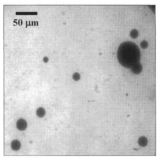
\includegraphics[width=\textwidth]{oleds/dark_spot}
    \caption{}
    \label{fig:oleds_dark_spot}\par\vfill
    \end{subfigure}
    \begin{subfigure}{.4\textwidth}
    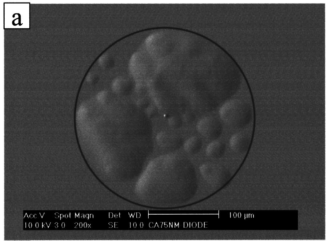
\includegraphics[width=\textwidth]{oleds/bubbles}
    \caption{}
    \label{fig:oleds_bubbles}
    \end{subfigure}
\caption{a. Dark spot in PL on an active device area, taken from \textcite{Kolosov2001}. b. Cathode bubbling where delamination has occurred under SEM, as shown in \textcite{Wang2002a}}
\end{figure}

One of the most widely observed and characterized degradation phenomena is the formation of dark spots.\supercite{Burrows1994,Aziz2004,Popovic2002,Liew2006}
This has been long attributed to delamination of the cathode, assisted by water and oxygen contamination or pinholes in the cathode.\supercite{Kolosov2001,Melpignano2005,Liao2007,Liew2006,Wang2002a}
Around an impurity under the cathode, a hot spot, or a cathode pinhole, the metal starts to delaminate from the underlying organic stack, forming a bubble.\supercite{Liao2007,Shin2006,Scott1996}
The field distribution around these dark spots creates high current around the edges, creating local high brightness regions.
This causes the dark spot to grow at an accelerated rate, further accelerating degradation.\supercite{Shin2006,Cumpston1997,Scott1996}

Despite the long history and understood mechanism, dark spots continue to be a major problem in manufacturing of large area lighting panels.\supercite{Giebink2017a}
The methods for preventing dark spots are largely understood, though control can be difficult.
It has been found that carefully controlling vacuum levels along with oxygen and moisture exposure during manufacture helps to prevent dark spot formation from oxygen and moisture under the cathode.
After manufacturing, oxygen and moisture can still get into the device through pinholes in the cathode, but this can be mitigated by careful packaging under a nitrogen environment.
For long lived devices, the addition of a moisture desiccant within the packaging further decreases dark spot formation.

\subsubsection{Exciton and Polaron}\label{sec:oleds_deg_mech_physics}

Most degradation mechanisms within a device are facilitated by the exciton and polaron population.\supercite{Bangsund2018,Scholz2015,Giebink2008a,Giebink2009a,Zhang2016,So2010}
These excited particles within the device provide the excess energy that is responsible for breaking bonds and facilitating the chemical processes that cause molecular degradation.
Reducing the exciton density by expanding the exciton recombination zone has been shown to extend lifetime.\supercite{Bangsund2018,Zhang2014,Wu2016,Chin2005,Lee2006,Chwang2002,Han2016,Lee2005a,Brown2004,Choong2000,Liu2004}
Despite this knowledge, high exciton densities are still often needed due to high brightness of devices, which can not be fully counteracted by continuing to extend the recombination zone.
In fact, most reduction in lifetime with brightness is attributed to increased exciton and polaron density.\supercite{Scholz2015}
In addition, it is often suggested that current is not uniform and typically confined to narrow pathways through the device.\supercite{Shen2015}
This causes locally high exciton and polaron densities, even with well designed injection and transport for a wide RZ.



\subsubsection{Interfaces}

Some devices have shown sensitivity to charges and excitons at material interfaces within devices.\supercite{Hershey2016,Wang2013}
Through single carrier device investigation, some materials have been shown to be sensitive to conduction of one type of carrier.\supercite{Aziz1999}
In other cases, a buildup of charge or exciton density can occur at an interface, greatly increasing the degradation rate locally at the interface.\supercite{Kondakov2003,Matsumura2003}
This type of degradation can result in the formation of Non-Radiative Recombination Centers (NRRCs).\supercite{Kondakov2007b,Kondakov2008,Kondakov2003,Kondakov2007d}
NRRCs are cites, typically of degraded molecules, that are able to recombine electrons and holes through a dark state who's emission is not seen.
The higher density of trapped charge at an interface can lead to formation of exciplex and transport layer excitons at the interface.  \supercite{Wang2013}
Transport layer excitons can be detrimental to device behavior due to their UV energies, especially when combined with polarons, leading to bimolecular quenching and hot excitons that can be more damaging than the presence of excitons or polarons on their own.

Interfacial degradation is also an exciton and polaron driven process, but bares the critical distinction of sensitivity to location.  
In materials with known interface and single carrier sensitivity, it is important to engineer the exciton profile away from these interfaces to extend lifetime, as shown in my work, \textcite{Hershey2016}, discussed in Chapter \ref{sec:decoupling_applications}.
This is contrary to the typical thought that only a broad recombination zone is important, discussed in the previous section.
Some devices even show sensitivity to both exciton density and recombination zone position, again, discussed in \ref{sec:decoupling_applications}.







\subsection{Luminance Scaling}\label{sec:luminance_scaling}
For commercially relevant devices, where the time to reach 50\% of the initial luminance, $t_{50}$ can be tens of thousands of hours, it is impractical to test devices under their intended operating conditions.
Instead, lifetime testing can be done at an increased luminance from the true operating condition.\supercite{Scholz2015}
This can dramatically reduce the testing time of devices.
The lifetime at other luminances can then be found using the scaling relation

\begin{equation}
L_0^n t_x=C
\label{eqn:luminance_scaling}
\end{equation}

where $L_0$ is the initial luminance, $n$ is a scaling factor characteristic to the device, and $C$ is a constant.
To utilize this relation, several lifetimes are obtained at luminances above the operating condition in order to experimentally obtain a value for $n$.
Subsequently, the lifetime of interest can then be extrapolated.

While widely used and observed, caution should be observed in the application of this relation.  
A variety of degradation mechanisms have been attributed to OLED behavior, as discussed in Section \ref{sec:degradation_mechanisms}.
All of these mechanisms are subject to different temporal dependences and have a variety of degrees of understanding to their functional dependence on time and luminance.
At different luminances, different mechanisms may be dominant.
For example, single excitonic processes may be dominant at low luminance, but may be overtaken by a bimolecular process at high luminance.
The fact that OLEDs are frequently subject to several degradation mechanisms throughout the decay only further complicates the issue.
The very idea of scaling law for all devices and at all current densities is unsound, and should be treated as a loose prediction.
Over and underestimates of lifetimes using this relation are observed when trying to predict actual lifetimes.\supercite{Meerheim2006,Fry2005}


\subsection{Analysis Techniques}\label{sec:degradation_analysis}

To expand on the luminance as a function of time, various analytical techniques are used to illuminate the degradation mechanisms.
These can largely be divided into chemical analysis, modeling, and spectral characterization.
These techniques offer valuable and unique insight, and are often used in combination for degradation analysis.

\subsubsection{Chemical Analysis}

\begin{figure}[ht]
\centering
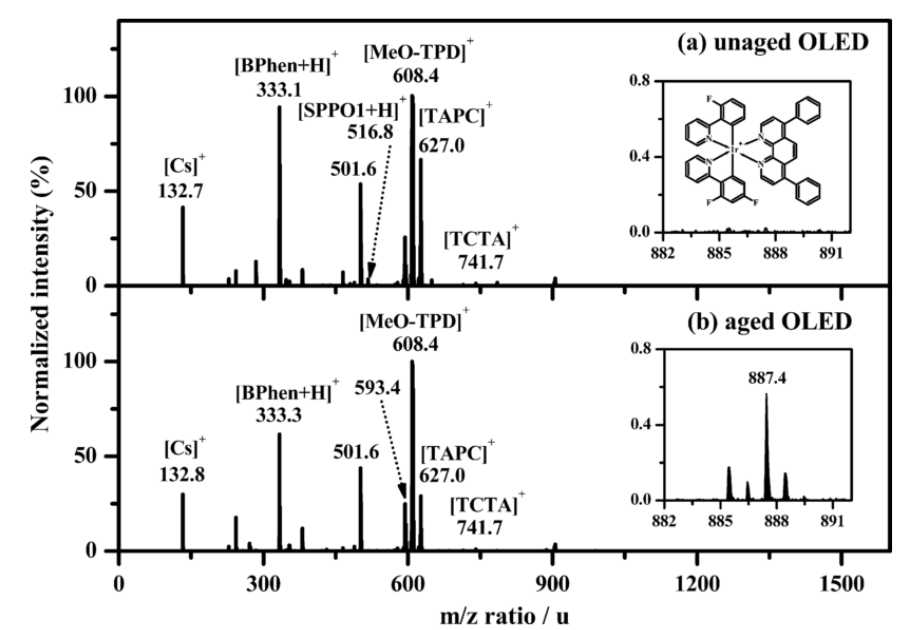
\includegraphics[width=.8\textwidth]{oleds/mass_spec}
\caption{Mass spectroscopy data taken from \textcite{Seifert2013b}}
\label{fig:oleds_mass_spec}
\end{figure}

Perhaps the most obvious approach is to look directly at the chemical composition of degradation products and use this to inform on what molecules are degrading.
A standard approach for doing this is Laser desorption/ionization time-of-flight mass spectroscopy (LDI-TOF-MS).\supercite{Moraes2011,DeMoraes2011,Seifert2013b}
With this technique, a laser is used to ionize the sample material, and time-of-flight is used to characterize the molecular weight to charge ratio.  
An example of this data can be seen in Figure \ref{fig:oleds_mass_spec}, taken from \textcite{Seifert2013b}.
Here, an unaged and aged sample are compared and peaks from known source material are identified.
Differences that are seen are attributed to degradation, and can be compared to the expected spectra of proposed degradation products.
In this case, a BPhen and FIr6 molecule have combined to form a new molecule.
It is important to note that despite degradation to ~15\% of the initial luminance, the molecular signatures of degradation products are extremely weak, as seen by the scale on the inset in Figure \ref{fig:oleds_mass_spec}.
This is a common problem for chemical techniques.
In devices, the active material stack is only a few monolayers thick and small amounts of degradation product can have a large impact.
Given the extremely low concentration and limited sample material, it can be difficult to do chemical analysis.
Even at heavy degradation, if several degradation products are present, none may be in high enough concentration to be observed.
Despite this drawback, understanding of results is very straight forward, making this a promising technique.

High performance liquid chromatography (HPLC) can also be used to view degradation products.\supercite{Kondakov2007d,Sivasubramaniam2009}
In HPLC, sample products are dissolved in a solution and filtered through a distillation column.  
Components can be categorized based on their transit time through the column.
This technique offers similar results, but suffers from several drawbacks, namely that it can be difficult to dissolve all of the materials in a devices, and that identification of compounds requires a pure sample of the degradation product to serve as a calibration for the column.  

Despite the direct interpretation of results, chemical techniques do have several drawbacks.
First of all, these processes can be expensive and time consuming to perform, making it difficult to apply to large scale optimization of devices.
In addition, it does not provide any temporal resolution on a single device, since this is an entirely destructive technique.
This makes it difficult to understand any kinetic.

\subsubsection{Modeling}

Modeling efforts have been used to try to understand the functional dependence of exciton density dependence and attribute this to a material dependent rate constant.\supercite{Giebink2008a,Coburn2016a,Coburn2017,Peng2017}
All of these works model the exciton population as a function of time using the equation:

\begin{equation}
\frac{dN_{ex}(x,t,t')}{dt}=\gamma n(x,t,t')p(x,t,t')-\frac{N_{ex}(x.t.t')}{\tau}-K_{DR}Q(x,t')N(x,t,t')
\label{eqn:giebink_model_N}
\end{equation}

where $N_{ex}$ is the exciton density, $n,p$ are the electron,hole densities, $\gamma$ is the Langevin recombination rate, $\tau$ is the exciton lifetime, $K_{DR}$ is the defect quenching rate, and $Q$ is the defect concentration.  
In this model, $t$ is the short term dynamics, while $t'$ represents the degradation scale evolution of parameters.
The electron and hole populations are fixed to form a predetermined recombination zone shape.
The generated defects serve as first order quenchers to the exciton population, as well as trap states that modify the recombination zone along with charge densities.

\begin{equation}
\frac{dQ(x,t')}{dt'}=\left\{
\begin{array}{ll} K_X n(x,t'), & K_X p(x,t') \\  
K_XN(x,t') & \\
K_XN^2(x,t') & \\  
K_XN(x,t')n(x,t'), & K_XN(x,t')p(x,t') 
\end{array} \right.
\label{eqn:giebink_model_defects}
\end{equation}

Applying this model for each of these mechanisms independently, then comparing the fitted results should indicate the dominant defect generation process.
\textcite{Giebink2008a} find for their device that exciton-polaron processes are dominant, though this process is likely system dependent.
This model allows fitting of luminance and voltage behavior as a function of time and luminance, which are shown to be consistent.
However, this model has a large number of rate constants that cannot be measured independently, and is largely over-parameterized.  
Caution must be taken with these results as they do not suggest a unique explanation of the physics happening in the device.

\subsubsection{Spectral Characterization}

\begin{figure}[ht]
\centering
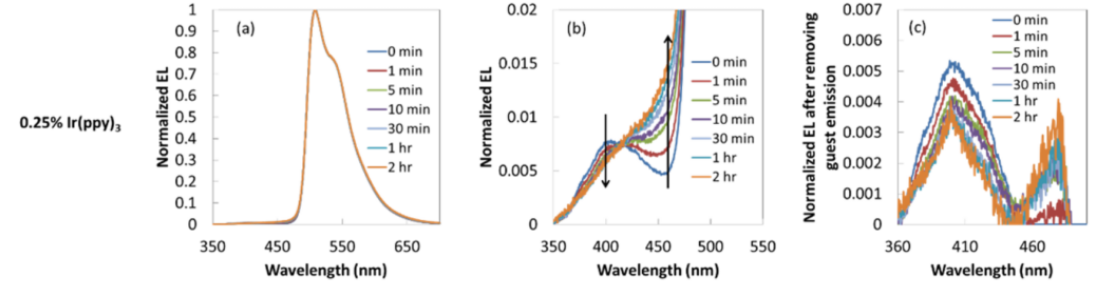
\includegraphics[width=.8\textwidth]{oleds/cbp_degradation}
\caption{Emission from \irppy and CBP, as reported by \textcite{Zhang2016} a. All emission, b. Emission shoulder, showing CBP emission, c. CBP emission with \irppy background subtracted.}
\label{fig:oleds_cbp}
\end{figure}

The electroluminescence spectra can also provide a large amount of information about the degradation state.\supercite{Scholz2015}
This is typically done in two schools of thought: intentional emission and observation of weakly emissive states.
Weakly emissive states and host emission have been used to characterize aggregation within the host and quest molecules.\supercite{Zhang2016,Wang2015a,Wang2014,Yu2017}
Within these studies, emission from the phosphorescent guest is characterized as a function of time, but careful inspection reveals weak emission from the host, as seen in Figure \ref{fig:oleds_cbp}.\supercite{Zhang2016}
In this figure, the weak CBP emission can be seen in the shoulder of the guest emission, and the losses during degradation characterized.
This study finds that host molecules are aggregating due to exciton and positive polaron interactions, accelerating degradation.

Another use of this technique is to track changes in the exciton recombination zone.  
This has been used in simplified bilayer devices where changes in relative peak intensities between two emissive species can indicate a shift of the RZ from one side of the device to the other.\supercite{Yu2017,Wang2010a}
This type of spectral characterization provides the temporal behavior of degradation that chemical analysis is lacking, but does not relate to physical processes within the device quantitatively, at least directly.
In fact, the understanding of physical mechanisms from the spectral changes can be far from straight forward.


Spectral characterization has been used recently as an extension of a modeling approach by \textcite{Coburn2017}, to interesting effect.
In this study, characterization of the exciton confinement within the emissive layer is desired.  
To study this, sensitizer doping layers are used outside of the emissive layer to probe for exciton leakage, using the red phosphor PtOEP, with emission shown in Figure \ref{fig:oleds_coburn}.
Using PtOEP, weak emission is seen in both cases, but is shown to increase in magnitude on the ETL side during degradation.  
\begin{wrapfigure}{r}{.5\textwidth}
\centering
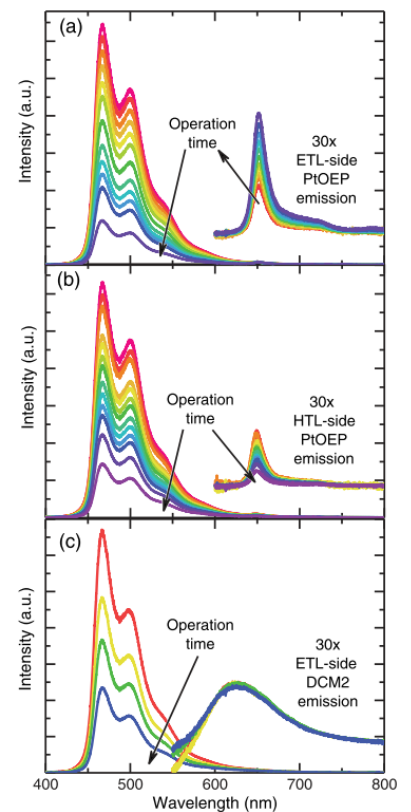
\includegraphics[width=.4\textwidth]{oleds/coburn}
\caption{Device emission spectra containing a. PtOEP sensitizer on the ETL side of the device, b. PtOEP sensitizer on the HTL side of the device, DCM2 sensitizer on the ETL side of the device.  Reproduced from \textcite{Coburn2017}}
\label{fig:oleds_coburn}
\end{wrapfigure}
This could indicate a decrease in exciton confinement, but would also be the case if holes were more efficiently leaking through the device.
To rule out hole leakage, a fluorescent dopant is used, which would not be able to receive diffusing triplet excitons.
Using DCM2, a fluorescent dopant, no increase in emission is seen, indicating that exciton confinement, not hole leakage, is responsible for this behavior.
This approach of using modeling in combination with a spectral technique is very promising at providing both more information to aid in modeling, and a more physical understanding to the spectral techniques.





\ifcsdef{mainfile}{}{\printbibliography}
\end{document}
